\section{Simulator and Results}
\subsection{Simulator}
\addtocounter{framenumber}{-1}
\begin{withoutheadline}
\begin{frame}{Simulator Architecture}


\setbeamercolor{block title}{bg=blue!30,fg=black}
\setbeamercolor{block body}{bg=blue!10,fg=black}
\setbeamertemplate{blocks}[rounded][shadow=false]

\begin{figure}[p]

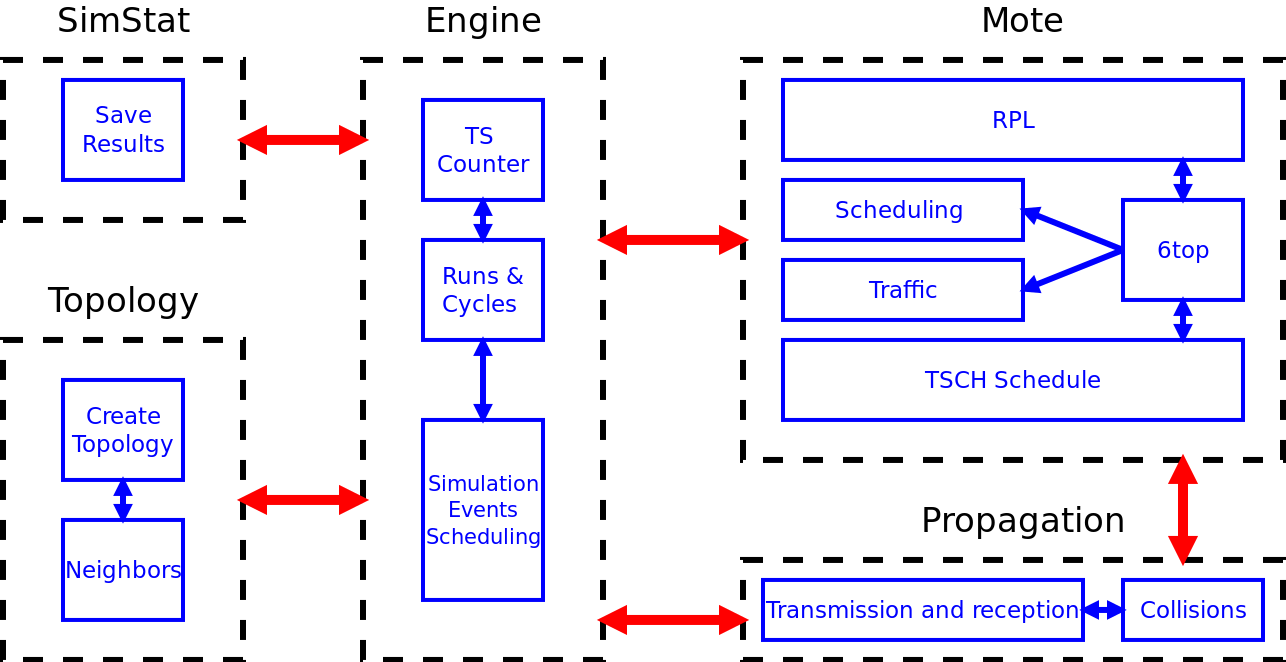
\includegraphics[width=\linewidth]{figures/SIM.png}

\end{figure}



\end{frame}
\end{withoutheadline}

\begin{withoutheadline}
\begin{frame}{Simulation Parameters}


\setbeamercolor{block title}{bg=blue!30,fg=black}
\setbeamercolor{block body}{bg=blue!10,fg=black}
\setbeamertemplate{blocks}[rounded][shadow=false]

\begin{center}
\begin{tabular}{l*{1}{c}r}
Parameter              & Value  \\
\hline
Number of Motes & $100$ \\
Number of cycles per run     & $1000$ \\
Number of runs per simulation     & $1000$ \\
Timeslot duration    & $10ms$ \\
Slotframe length     & $101$\\
Number of channels   & $16$ \\
Area            & $1Km\times1Km$ \\
Topology constraint     & $\geq$ 3 neighbors with PDR $50\,\%$ \\
Radio sensitivity           & $-97$ dBm \\
Radio range     & 100m \\
Traffic & 1 packet/node each 10 cycles 
\end{tabular}
%\captionof{table}{Simulator Parameters} \label{tab:para} 
\end{center}





\end{frame}
\end{withoutheadline}


\subsection{ Results}
\addtocounter{framenumber}{-1}
\begin{withoutheadline}
\begin{frame}{Comparison with random scheduling}

\begin{figure}[p]

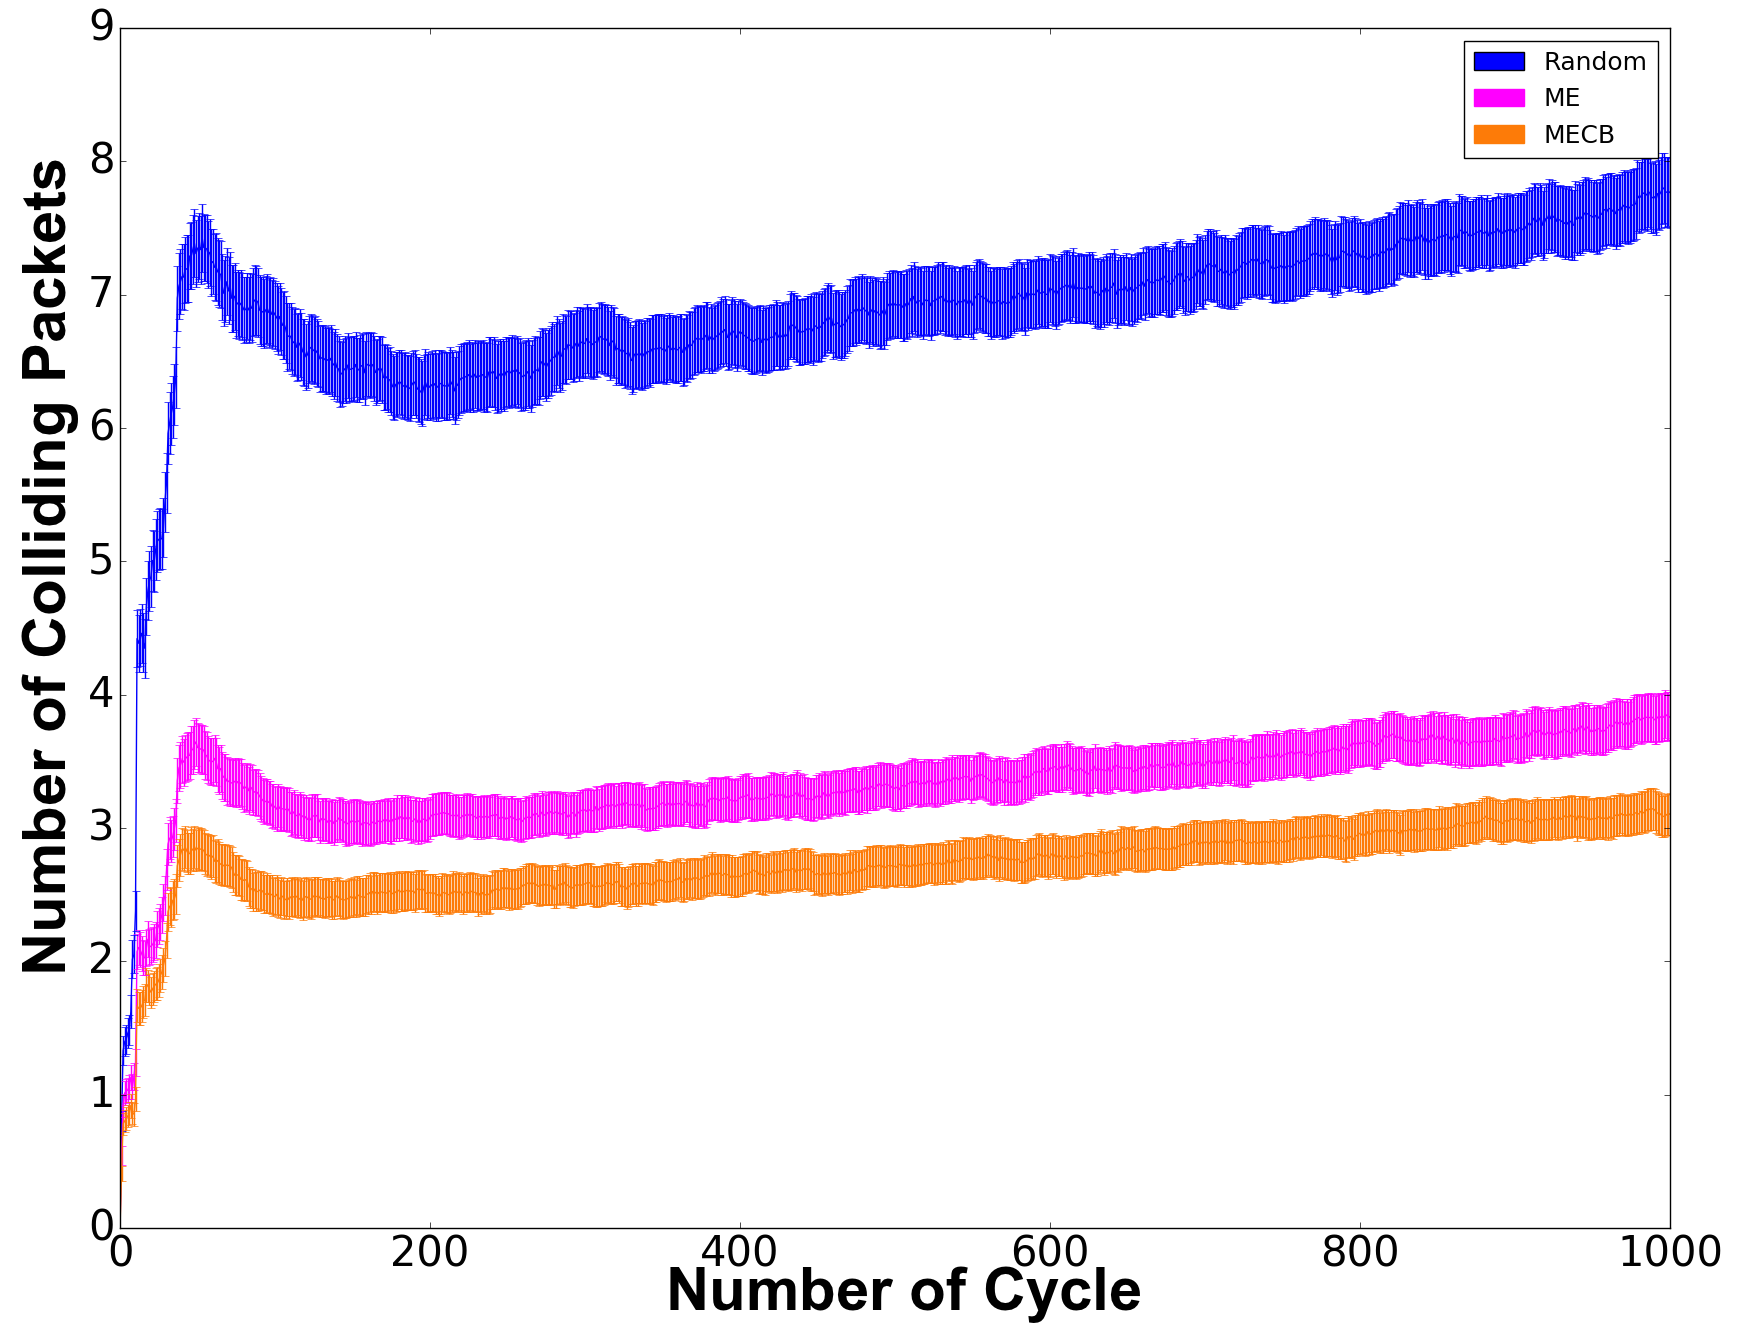
\includegraphics[width=\linewidth]{figures/graph1.png}

\end{figure}



\end{frame}
\end{withoutheadline}

\begin{withoutheadline}
\addtocounter{framenumber}{-1}
\begin{frame}{Comparison with random scheduling}

\begin{figure}[p]


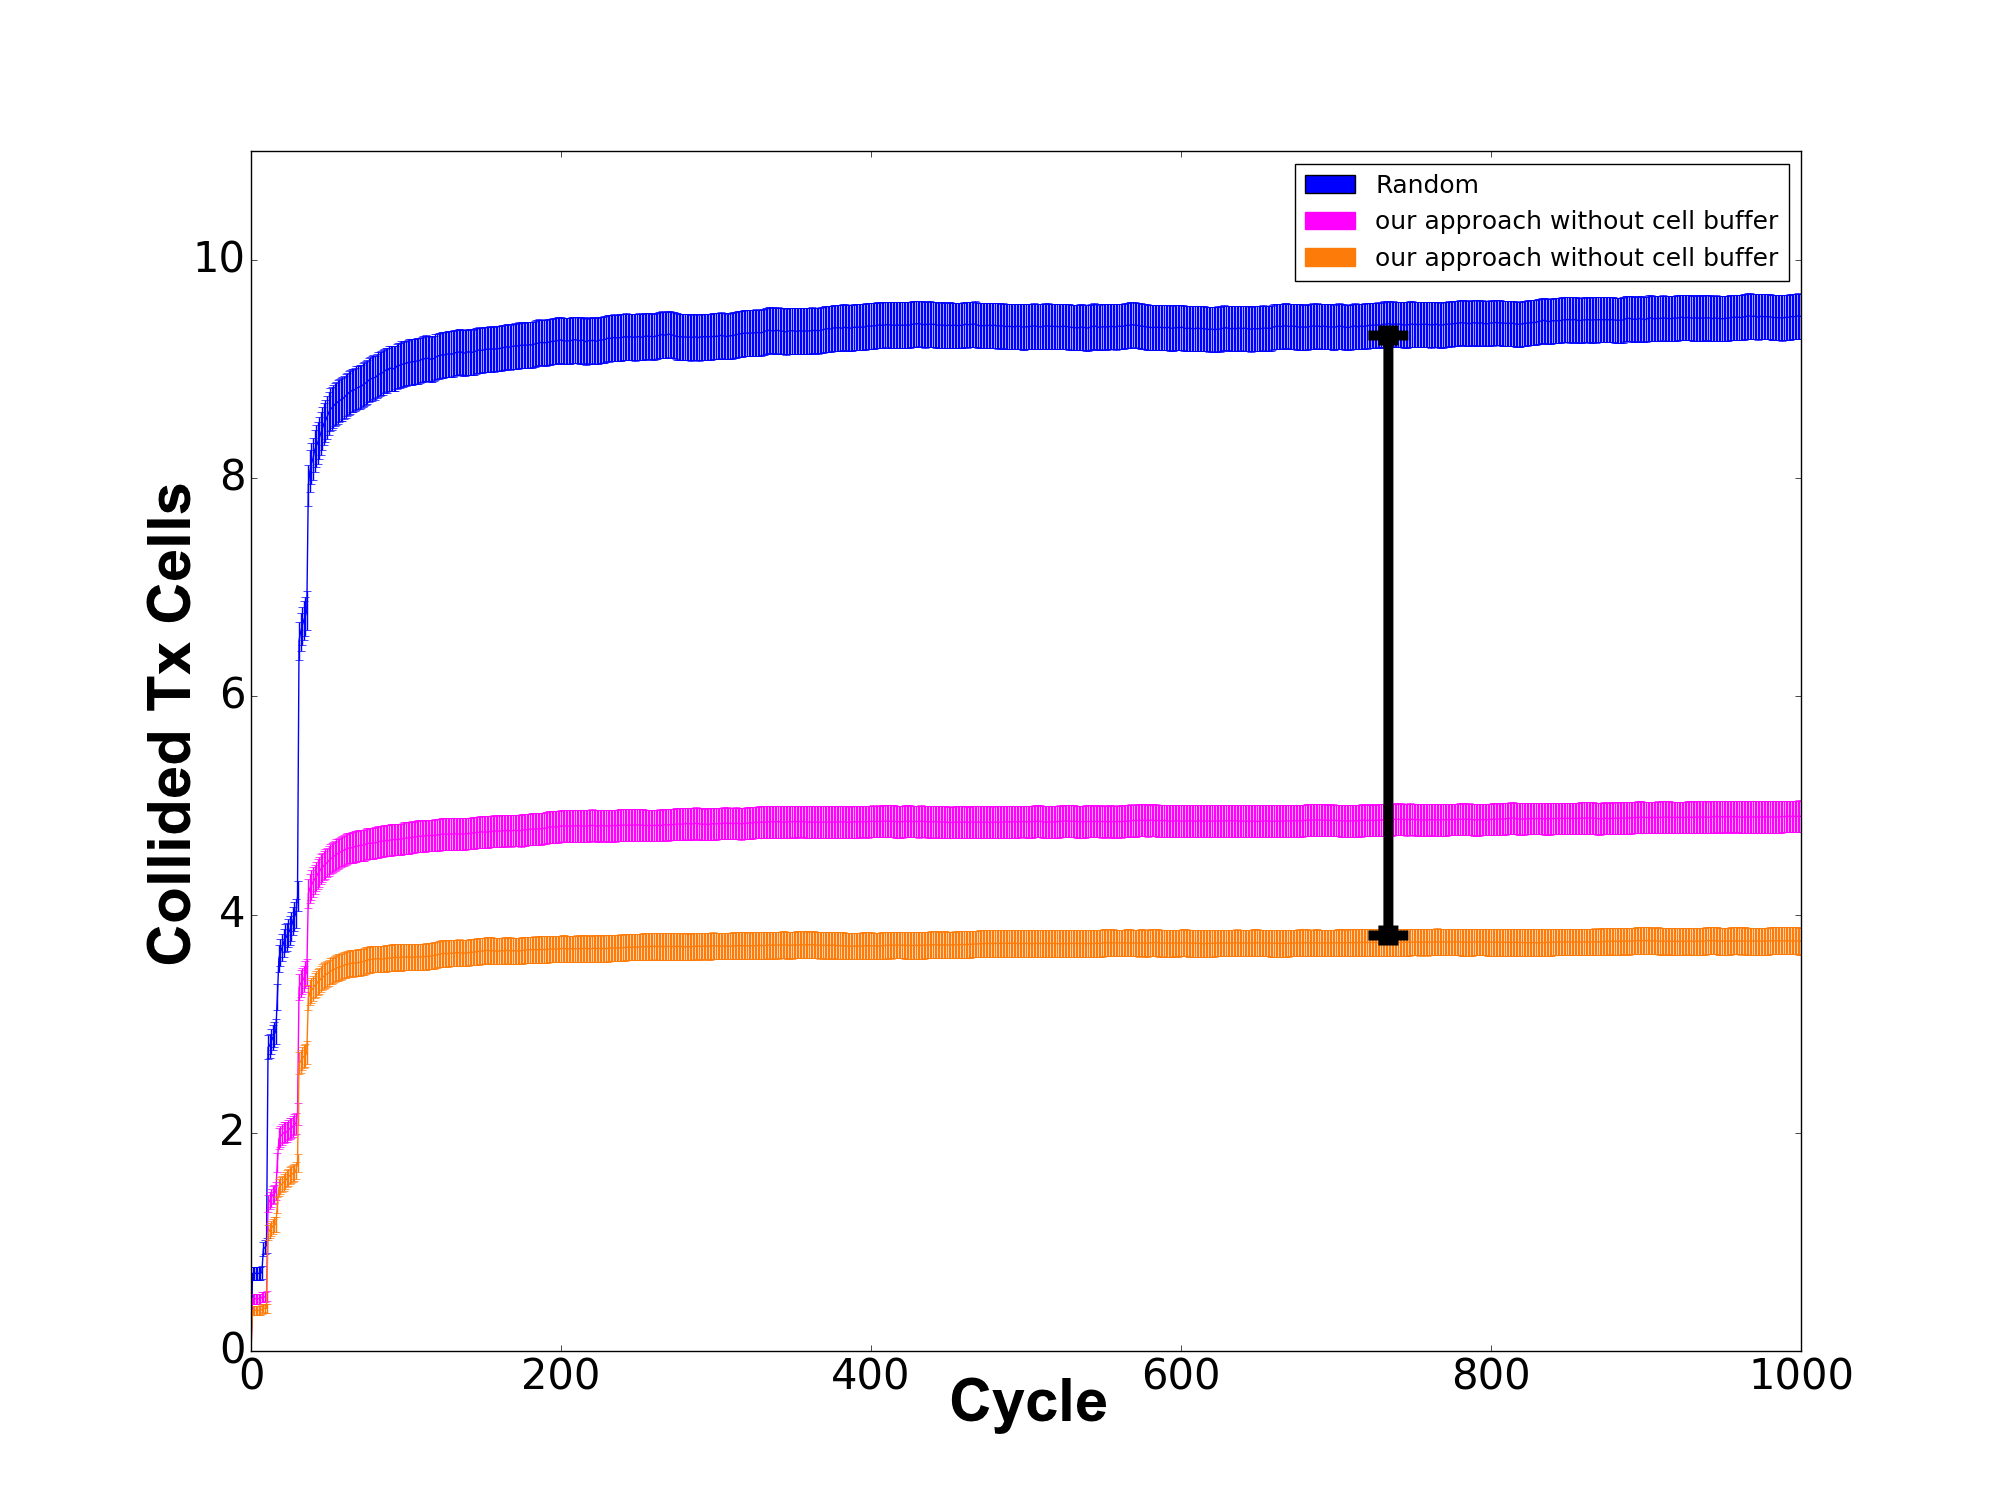
\includegraphics[width=\linewidth]{figures/graph1-1.png}
\end{figure}



\end{frame}
\end{withoutheadline}

\begin{withoutheadline}
\addtocounter{framenumber}{-1}
\begin{frame}{Comparison with random scheduling}

\begin{figure}[p]


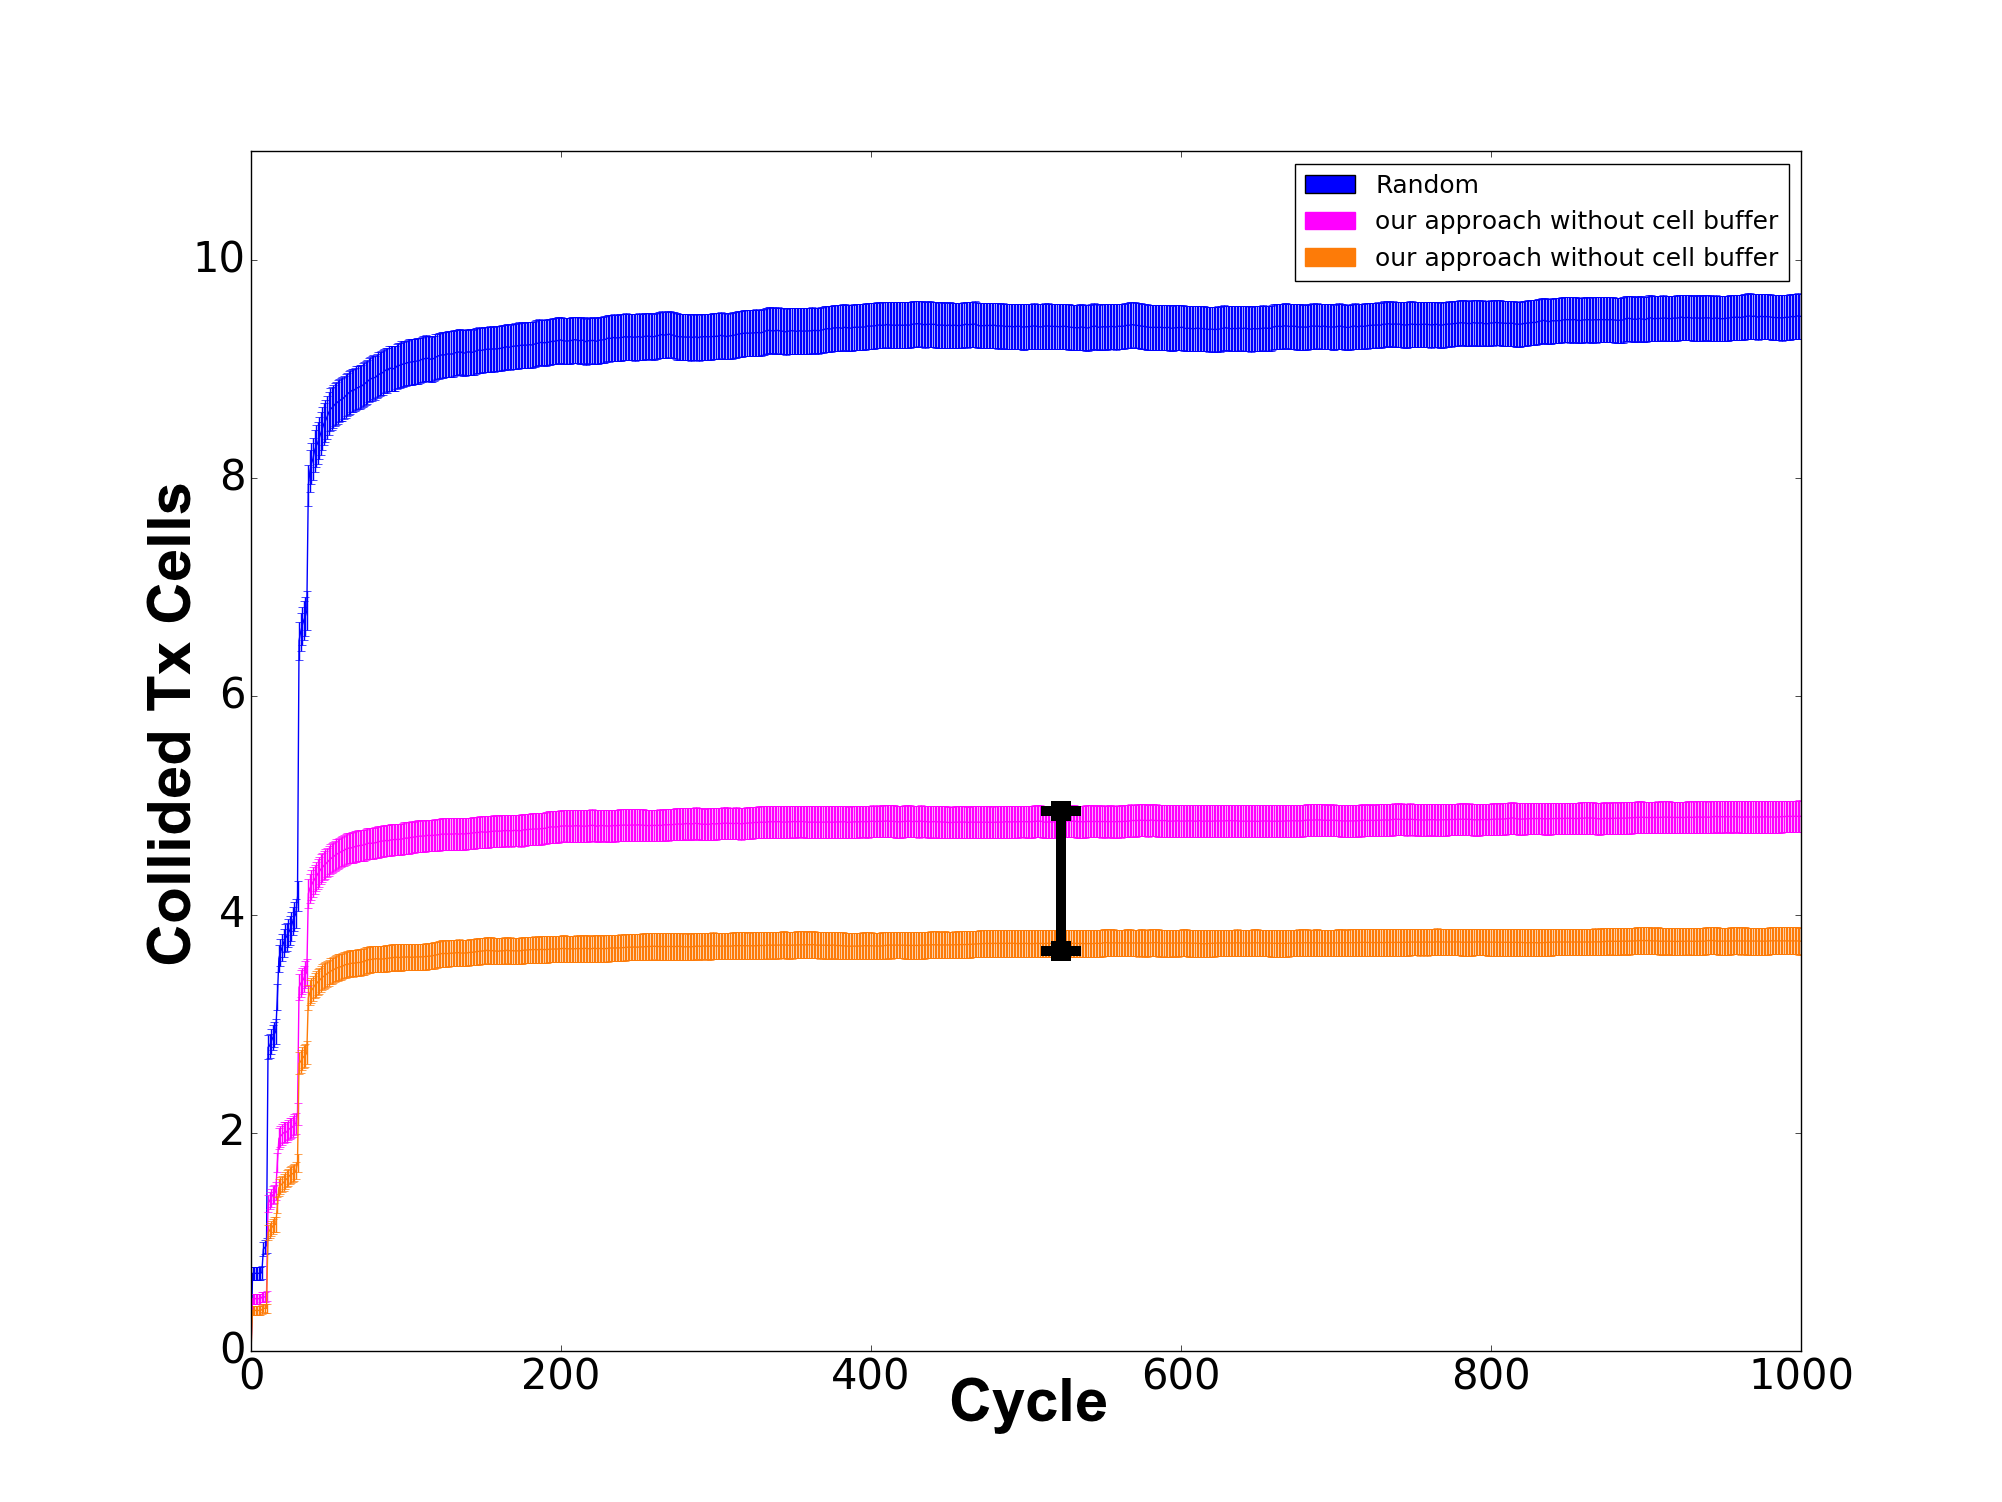
\includegraphics[width=\linewidth]{figures/graph1-2.png}
\end{figure}



\end{frame}
\end{withoutheadline}


\begin{withoutheadline}
\begin{frame}{ Results}


\setbeamercolor{block title}{bg=blue!30,fg=black}
\setbeamercolor{block body}{bg=blue!10,fg=black}
\setbeamertemplate{blocks}[rounded][shadow=false]


\begin{block}{Collision reasons}

    \begin{itemize}
    \item The lost 6top transactions. 
\item Special Case That Induce Collisions.
    
     
    
    \end{itemize}
    \end{block}

\centering
\begin{figure}[p]

\item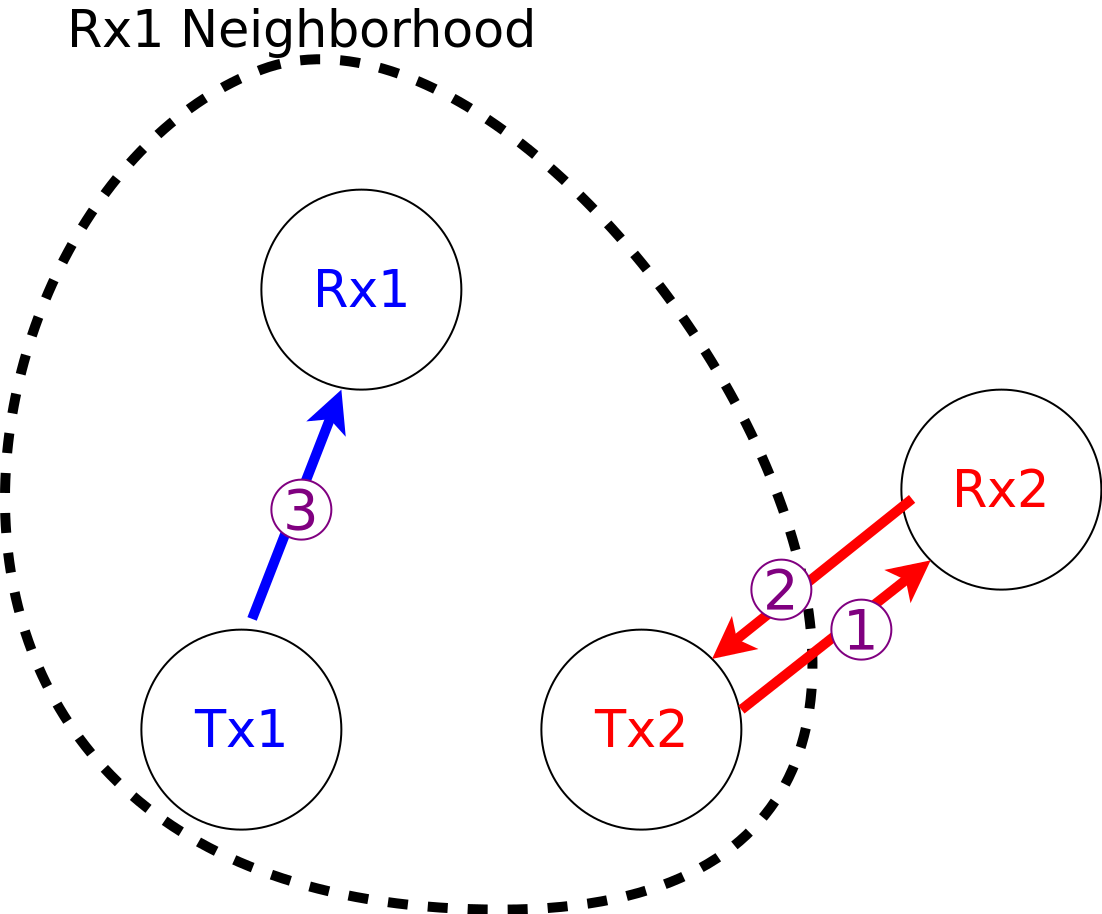
\includegraphics[width=0.4\linewidth]{figures/pro.png}
\end{figure}

\end{frame}
\end{withoutheadline}


\begin{withoutheadline}
\begin{frame}{Housekeeping Approach}


\setbeamercolor{block title}{bg=blue!30,fg=black}
\setbeamercolor{block body}{bg=blue!10,fg=black}
\setbeamertemplate{blocks}[rounded][shadow=false]
\begin{minipage}[t]{0.48\linewidth}

\begin{block}{Collision in Dedicated Cells}
    \begin{itemize}
    \item Housekeeping approach and cell relocation.
    \item Tx housekeeping. 
    \item<4-> Rx housekeeping. 
    \item<6-> Dealing with collisions after they occur. Good idea ?
    
    \end{itemize}
    \end{block}
\end{minipage}\hfill
\begin{minipage}[t]{0.48\linewidth}
\begin{figure}[p]
 \only<1>{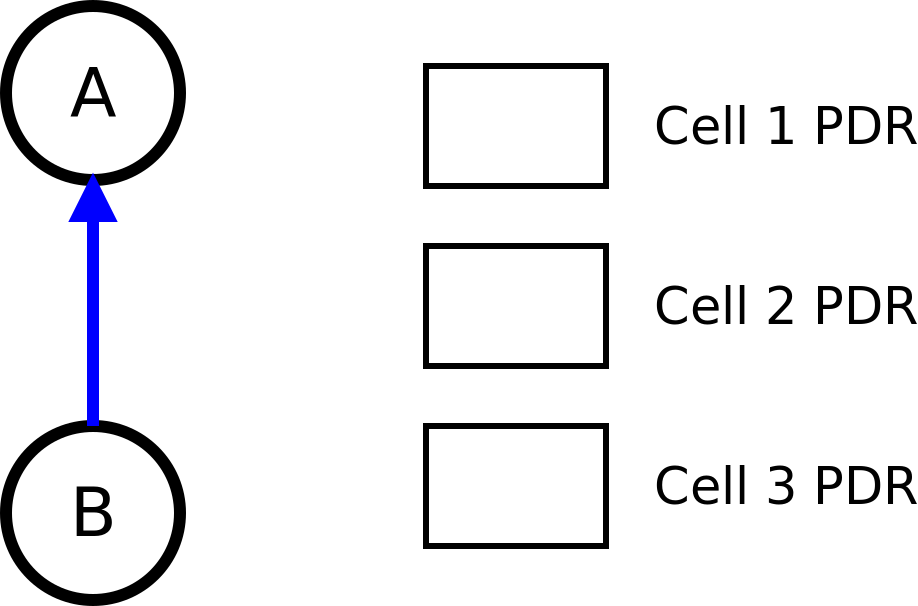
\includegraphics[width=\linewidth]{figures/hk1.png}}
 \only<2>{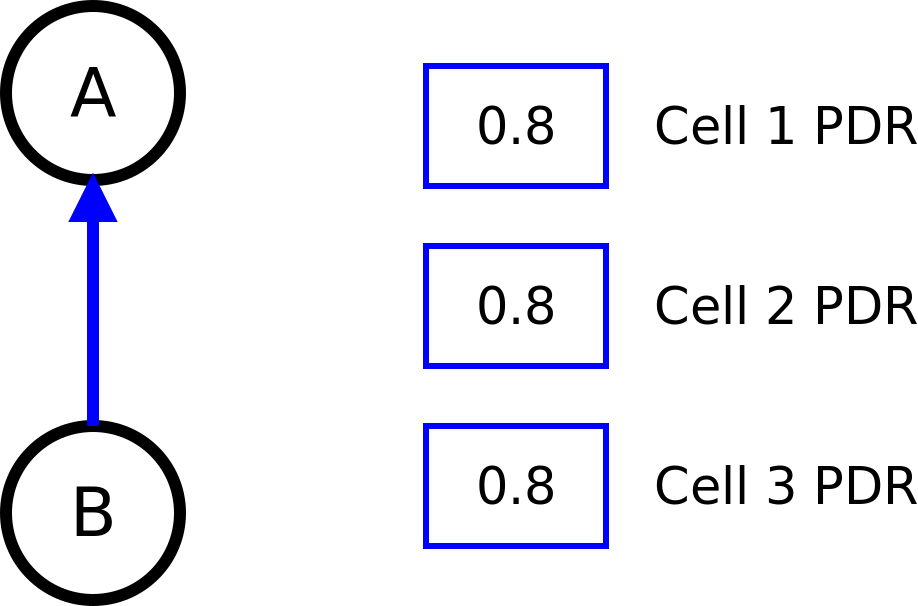
\includegraphics[width=\linewidth]{figures/hk2.png}}
  \only<3>{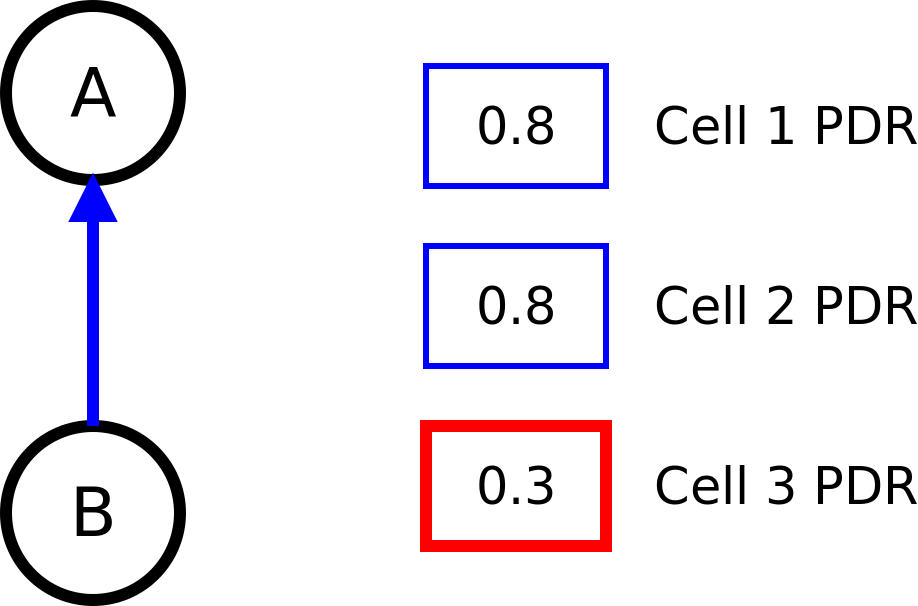
\includegraphics[width=\linewidth]{figures/hk3.png}}
  \only<4>{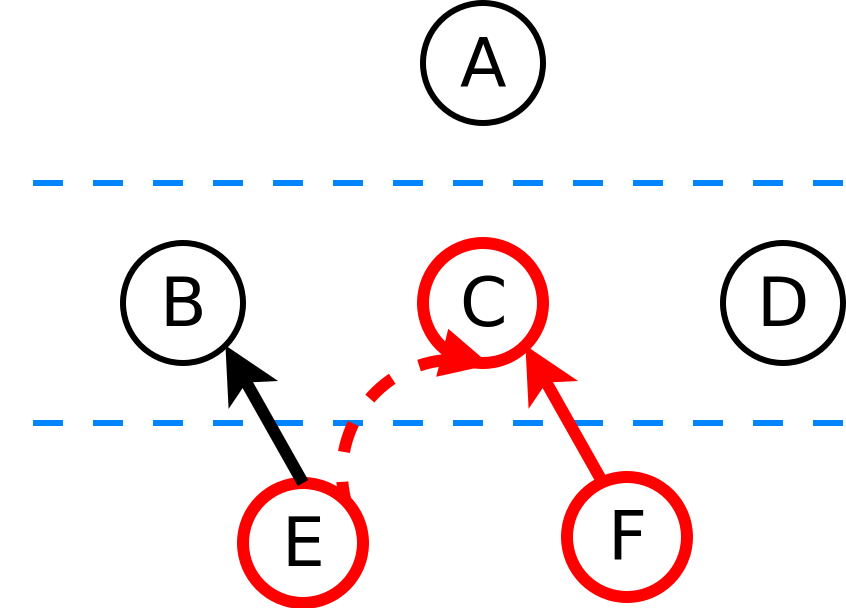
\includegraphics[width=\linewidth]{figures/rx1.png}}
  \only<5->{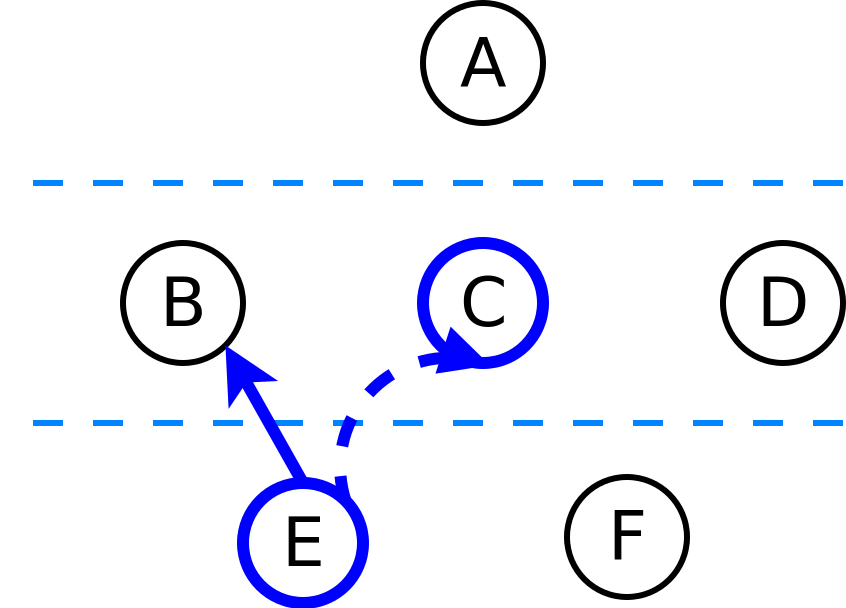
\includegraphics[width=\linewidth]{figures/rx2.png}}
  
\end{figure}
\end{minipage}

\end{frame}
\end{withoutheadline}


\begin{withoutheadline}
\begin{frame}{Comparison with Housekeeping }

\begin{figure}[p]

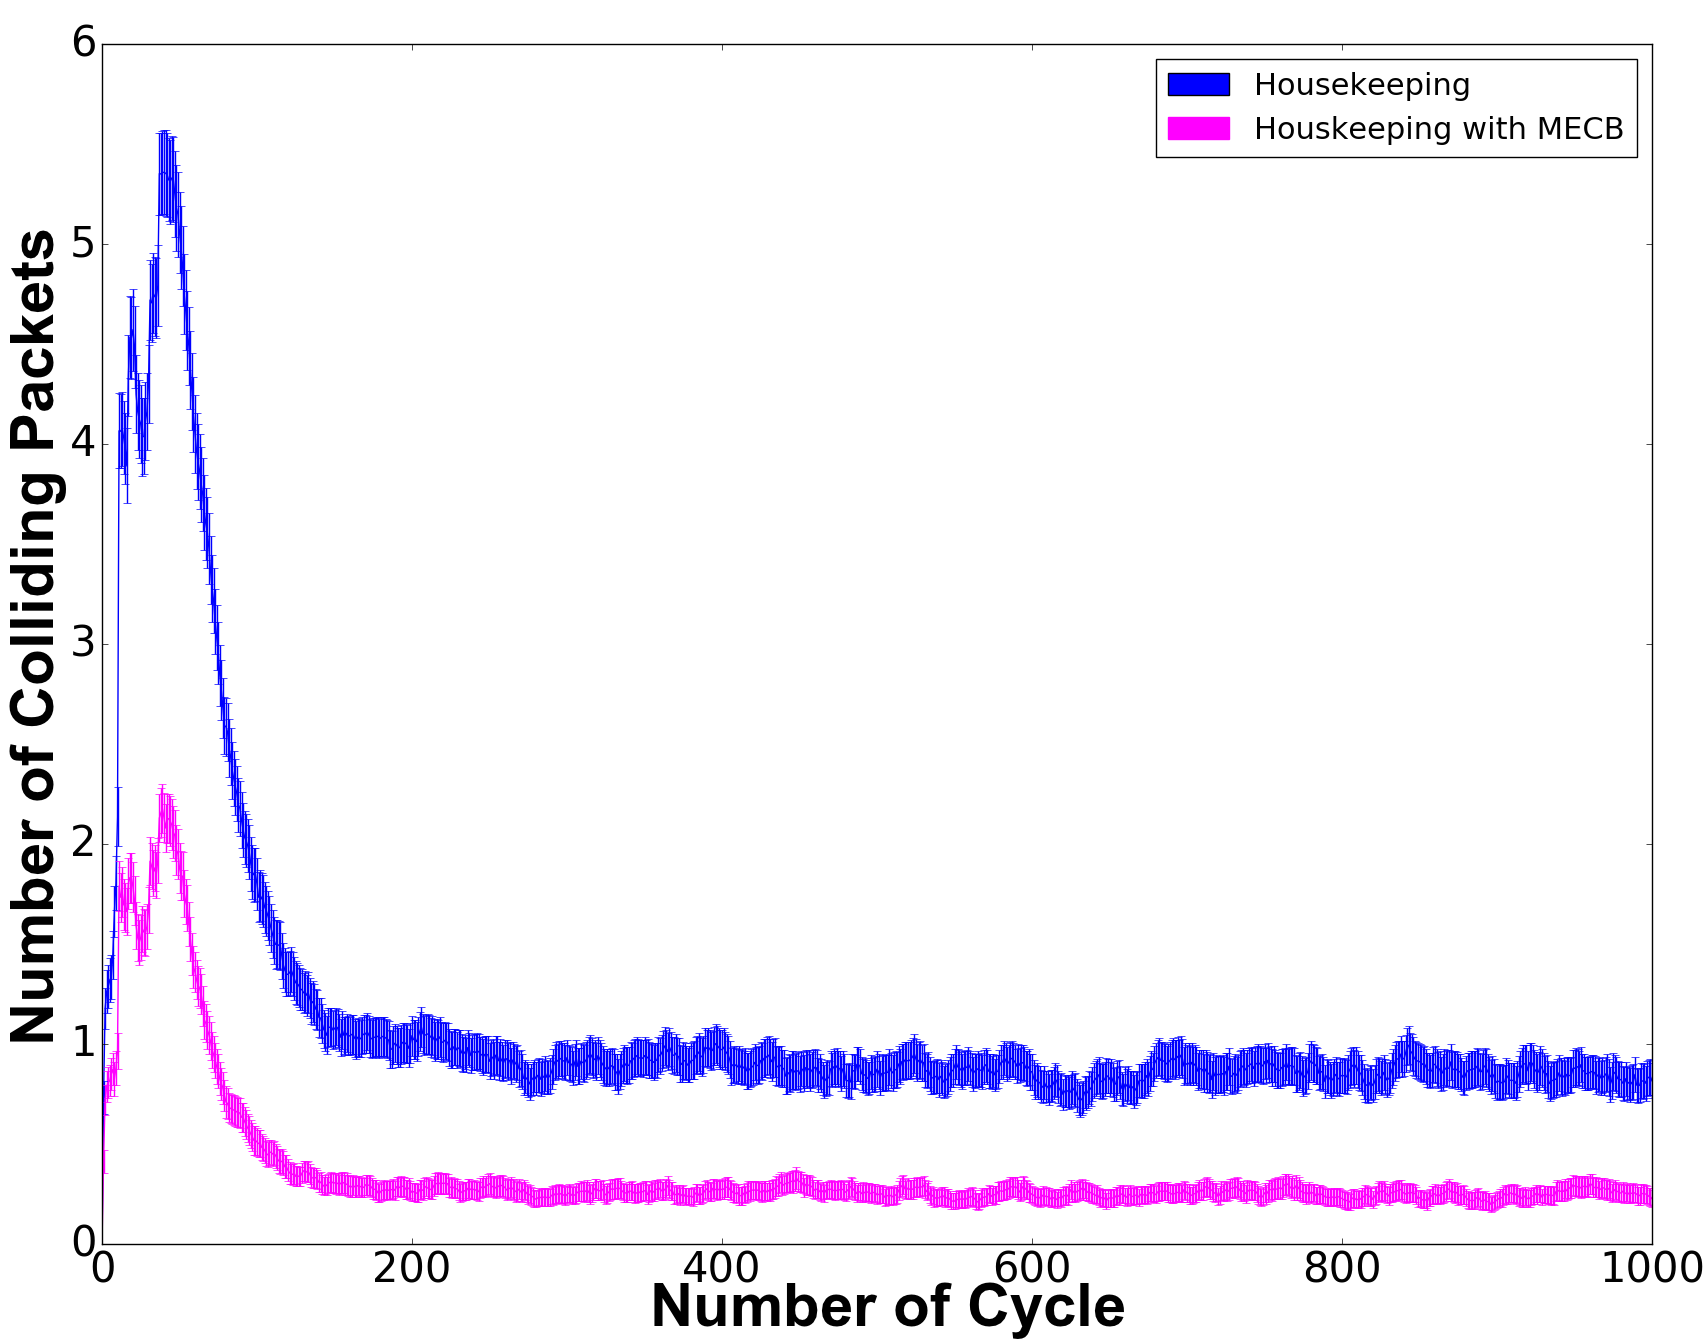
\includegraphics[width=\linewidth]{figures/graph2.png}
%\caption{Simulation of the Number of Collided Tx Cells as Function of Cycle Number (Time) - comparison with the housekeeping approach}
\end{figure}



\end{frame}
\end{withoutheadline}



%%%%%%%%%%%%%%%%%%%%%%%SUMMARY%%%%%%%%%%%%%%
\section{Summary and Contributions}

\begin{withoutheadline}
\begin{frame}{Summary}
  \begin{itemize}
  \item
    Our implementation introduce  \alert{no overhead } in the network.
  \item
    The implementation \alert{achieved 60\% reduction} in the number of collided Tx cells.
  \item The Combination of Our approach and Housekeeping accomplish an \alert{ almost collision free dedicated cells}.
  \end{itemize}
  
  \begin{itemize}
  \item
    Outlook
    \begin{itemize}
    \item
     Our goal is to reach a place were we have collision free network, using more complex methods.
    \item
      Our perspective in this project was work on 6top, but our next steps is to study the effects of traffic in the protocols performances.
    \end{itemize}
  \end{itemize}
\end{frame}
\end{withoutheadline}


\begin{withoutheadline}
\begin{frame}{Contributions}
  \begin{itemize}
  \item Understanding the simulator code.
  \item Optimizing, and implementing on top of this code.
  \item Designing the proposed mechanisms, and enhancing them.
  \item Publishing a poster in Computational sciences days in Grenoble, organized by LabEx PERSYVAL-Lab.
  \item Submitting a paper to Wimob 2017 conference. 
  \end{itemize}
  \begin{figure}[p]
\centering

\includegraphics[width=.5\linewidth]{figures/per.png}

\end{figure}
\end{frame}
\end{withoutheadline}